% !TEX TS-program = lualatex
% Краткая статья-отчет по НИР.
% Файл рассчитан на размещение в корне репозитория:
% https://github.com/Dima12101/SPbU-Phd-LaTeX-Dissertation
% Сборка: lualatex nir_report_article_style.tex
\documentclass[a4paper,14pt]{extarticle}

\usepackage{fontspec}
\usepackage{polyglossia}
\setmainlanguage{russian}
\setotherlanguage{english}
\defaultfontfeatures{Ligatures=TeX}
\IfFontExistsTF{Times New Roman}{%
  \setmainfont{Times New Roman}
  \newfontfamily\cyrillicfont{Times New Roman}
}{%
  \IfFontExistsTF{Liberation Serif}{%
    \setmainfont{Liberation Serif}
    \newfontfamily\cyrillicfont{Liberation Serif}
  }{%
    \setmainfont{DejaVu Serif}
    \newfontfamily\cyrillicfont{DejaVu Serif}
  }%
}
\IfFontExistsTF{Liberation Mono}{%
  \newfontfamily\cyrillicfonttt{Liberation Mono}
}{%
  \newfontfamily\cyrillicfonttt{DejaVu Sans Mono}
}

\usepackage{geometry}
\geometry{left=25mm,right=20mm,top=20mm,bottom=20mm}
\usepackage{setspace}
\onehalfspacing
\usepackage{indentfirst}
\setlength{\parindent}{1.25cm}
\usepackage{microtype}
\usepackage{graphicx}
\usepackage{booktabs}
\usepackage{array}
\usepackage{tabularx}
\usepackage{float}
\usepackage{caption}
\usepackage{amsmath,amssymb}
\usepackage{enumitem}
\usepackage{cite}
\renewcommand{\citedash}{-}
\usepackage{hyperref}
\hypersetup{hidelinks}

\graphicspath{{Dissertation/images/}{Dissertation/images/results/}}

\newcommand{\methodname}{AMPLE-AMR}
\newcommand{\clustermethodname}{C-AMPLE-AMR}
\newcommand{\safeincludegraphics}[2][]{%
  \IfFileExists{#2}{\includegraphics[#1]{#2}}{%
  \IfFileExists{Dissertation/images/#2}{\includegraphics[#1]{Dissertation/images/#2}}{%
  \IfFileExists{Dissertation/images/results/#2}{\includegraphics[#1]{Dissertation/images/results/#2}}{%
  \fbox{\parbox{0.88\textwidth}{\centering Файл иллюстрации не найден: \texttt{\detokenize{#2}}}}}}}%
}

\newcommand{\keywords}[1]{\par\noindent\textbf{Ключевые слова:} #1\par}

\begin{document}

\begin{center}
{\large Санкт-Петербургский государственный университет}\par
\vspace{0.8em}
{\bfseries\Large Гибридный метод адаптивного распределения вычислительных задач автономных мобильных роботов в периферийной инфраструктуре}\par
\vspace{0.8em}
{\large Краткий отчет о научно-исследовательской работе в формате научно-технической статьи}\par
\vspace{0.8em}
\textbf{Аспирант:} Терещенко Дмитрий Владиславович\par
\textbf{Научный руководитель:} к.ф.-м.н., доц. Корхов В.\,В.\par
\textbf{Научная специальность:} 1.2.1 --- Искусственный интеллект и машинное обучение\par
\vspace{0.5em}
Санкт-Петербург, 2026
\end{center}

\begin{abstract}
\noindent В работе рассматривается задача распределения вычислительных задач автономных мобильных роботов между ограниченными периферийными вычислительными узлами. Такая задача возникает в роботизированных складах и других локальных киберфизических средах, где роботы генерируют неоднородный поток задач локализации, обработки сенсорных данных, распознавания объектов, перепланирования маршрутов и обмена телеметрией. Полностью бортовая обработка ограничена энергопотреблением, массой и тепловым режимом робота, а передача всех задач в удаленное облако не гарантирует требуемую задержку. Периферийные вычисления снимают часть этих ограничений, но превращают периферийные узлы в общий дефицитный ресурс, за который конкурируют задачи разных роботов~\cite{Chaari2022RobotOffloadingSurvey,Mao2017MECPerspective,Satyanarayanan2017Emergence,Shi2016Edge,Tahir2025EdgeRoboticsSurvey}.

Предложен гибридный метод \methodname{}, объединяющий VCG-подобный аукционный слой распределения задач и кооперативное многоагентное обучение с подкреплением для выбора операционных режимов периферийных узлов~\cite{Vickrey1961Counterspeculation,Clarke1971MultipartPricing,Groves1973IncentivesTeams,Rashid2018QMIX}. Аукционный слой используется как механизм внутренней координации и оценки внешнего эффекта назначения задачи, а обучаемый контур отвечает за долговременную адаптацию к изменению нагрузки, очередей, задержек и отказов. Для крупных конфигураций предложен вариант \clustermethodname{}, локализующий распределение внутри кластеров графа периферийной инфраструктуры. Реализован программный прототип и выполнена экспериментальная проверка в домене роботизированного склада. 
\end{abstract}

\keywords{автономные мобильные роботы; периферийные вычисления; распределение задач; VCG-механизм; многоагентное обучение с подкреплением; QMIX; роботизированный склад}

\section{Введение}

Автономные мобильные роботы (Autonomous Mobile Robot, AMR) в современных складских и производственных средах перестали быть только транспортными устройствами. Они выполняют вычислительно нагруженные операции, связанные с восприятием, навигацией, локализацией, обработкой данных с лидара и камеры, контролем безопасности, перестроением маршрутов и координацией с другими участниками системы. Рост числа роботов и плотности задач приводит к тому, что вычислительная инфраструктура становится самостоятельным объектом управления, а не вспомогательным фоном робототехнической системы~\cite{Fragapane2021AMRPlanning,Fragapane2024AMRMaterialHandling,Lackner2024AMRIntralogistics,Keith2024WarehouseAMRReview}.

\begin{figure}[h]
	\centering
	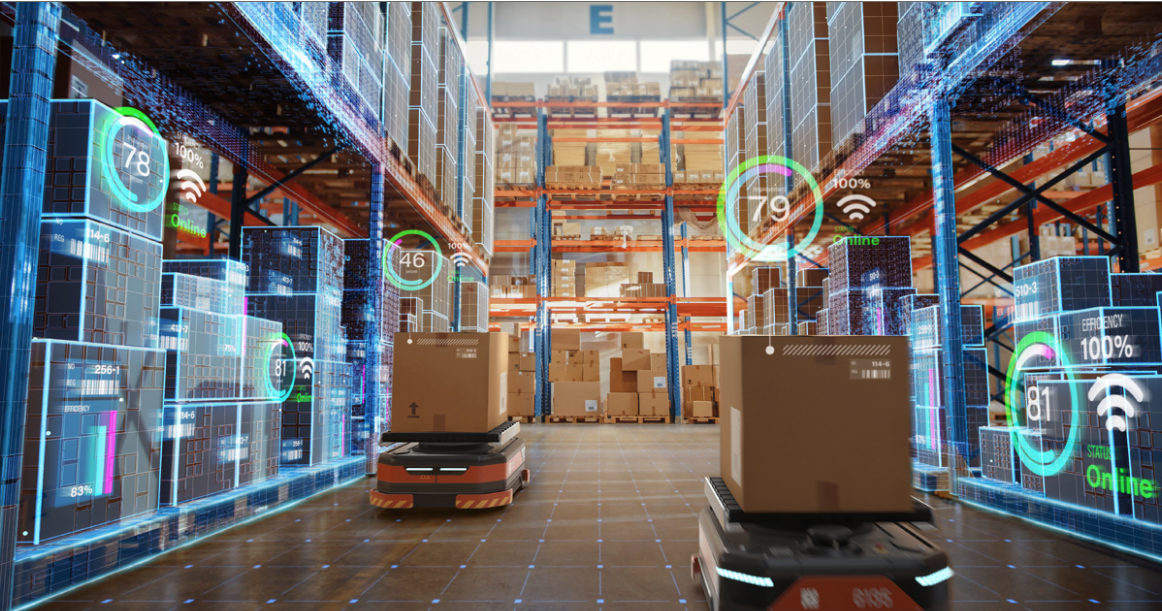
\includegraphics[width=14cm, height=8cm]{ch1_warehouse_robotics}
	\caption{Роботизированный склад}
	\label{img:ch1_warehouse_robotics}
\end{figure}

Возможны три базовые стратегии обработки данных. Первая стратегия состоит в выполнении задач на борту робота. Она минимизирует сетевую зависимость, но ограничена энергопотреблением, массой, стоимостью и тепловым режимом вычислительного модуля. Вторая стратегия состоит в передаче задач в удаленное облако. Она увеличивает доступную вычислительную мощность, но ухудшает предсказуемость задержки и создает зависимость от внешнего канала связи. Третья стратегия использует периферийные вычисления, размещая вычислительные ресурсы ближе к рабочей зоне роботов~\cite{Hu2012CloudRobotics,Wan2016CloudRobotics,Afrin2021CloudRoboticsSurvey,Shi2016Edge,Satyanarayanan2017Emergence,Groshev2023EdgeRoboticsReady}. Именно эта стратегия является наиболее естественной для локальных роботизированных складов, однако она порождает новую \textbf{проблему}: периферийные узлы сами являются ограниченным, неоднородным и динамически загруженным ресурсом.

\begin{figure}[h]
	\centering
	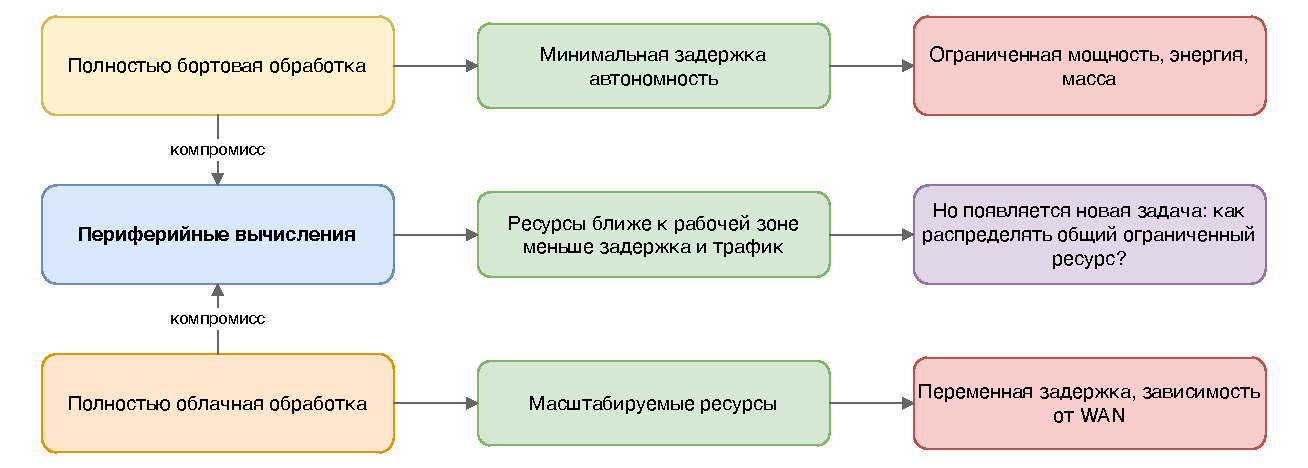
\includegraphics[width=0.95\textwidth]{ch1_edge_need_concept}
	\caption{Почему для AMR нужны периферийные вычисления?}
	\label{img:ch1_edge_need_concept}
\end{figure}

Следовательно, задача исследования состоит не только в том, чтобы назначить очередную задачу на ближайший или наиболее свободный узел. Необходимо учитывать дедлайны, приоритеты, задержки передачи, очереди, классы вычислительных задач, стоимость использования узлов, возможные отказы, пиковые волны нагрузки и внешний эффект назначения: задача, помещенная на один узел, изменяет доступность этого узла для остальных задач. Поэтому локально хорошее назначение может быть глобально невыгодным для системы.

\textbf{Цель выполненного исследования} --- разработать модель и метод адаптивного распределения вычислительных задач автономных мобильных роботов между периферийными узлами, в котором распределение общего ресурса остается формально интерпретируемым, а управление инфраструктурой адаптируется к динамике среды. Для этого предложен метод \methodname{}: аукционный слой формирует распределение задач и внутренние оценки внешнего эффекта, а обучаемая многоагентная политика управляет операционными режимами периферийных узлов.

\section{Исследовательский разрыв}

Существующие подходы к распределению вычислительных ресурсов на периферии можно условно разделить на четыре класса. Оптимизационные методы позволяют явно задать ограничения и критерий качества, но требуют достаточно полной информации о состоянии системы и могут быть чувствительны к масштабу задачи. Эвристические методы проще и быстрее, однако часто используют локальные правила и плохо описывают внешний эффект конкуренции за ресурс. Аукционные методы естественно выражают дефицит ресурса и конкуренцию участников, но в классической форме ориентированы на отдельный раунд распределения. Методы обучения с подкреплением способны учитывать долговременные последствия решений, но без дополнительной структуры могут терять интерпретируемость и превращать распределение ресурса в <<черный ящик>>~\cite{Luo2021ResourceScheduling,Djigal2022MLMECSurvey,Hortelano2023RLOffloadingSurvey,Peng2024DRLOffloadingSurvey,Qiu2022AuctionEdgeSurvey,Zhang2021MARLSurvey,Oroojlooy2023CoopReview,Ning2024MARLSurvey}.

Для рассматриваемой AMR-среды важна не замена одного класса методов другим, а разделение их ролей. Аукционный механизм должен отвечать за формальное распределение задач в текущем раунде, тогда как обучаемый контур должен отвечать за выбор режима работы узлов с учетом накопленной динамики. Такое разделение особенно важно в системе одного оператора: речь не идет о денежном рынке независимых владельцев роботов и узлов, но аппарат механизма Викри--Кларка--Гровса полезен как способ вычислить внутренние теневые цены и оценить внешний эффект использования ограниченного ресурса~\cite{Vickrey1961Counterspeculation,Clarke1971MultipartPricing,Groves1973IncentivesTeams,Qiu2022AuctionEdgeSurvey}.

\begin{figure}[h]
	\centering
	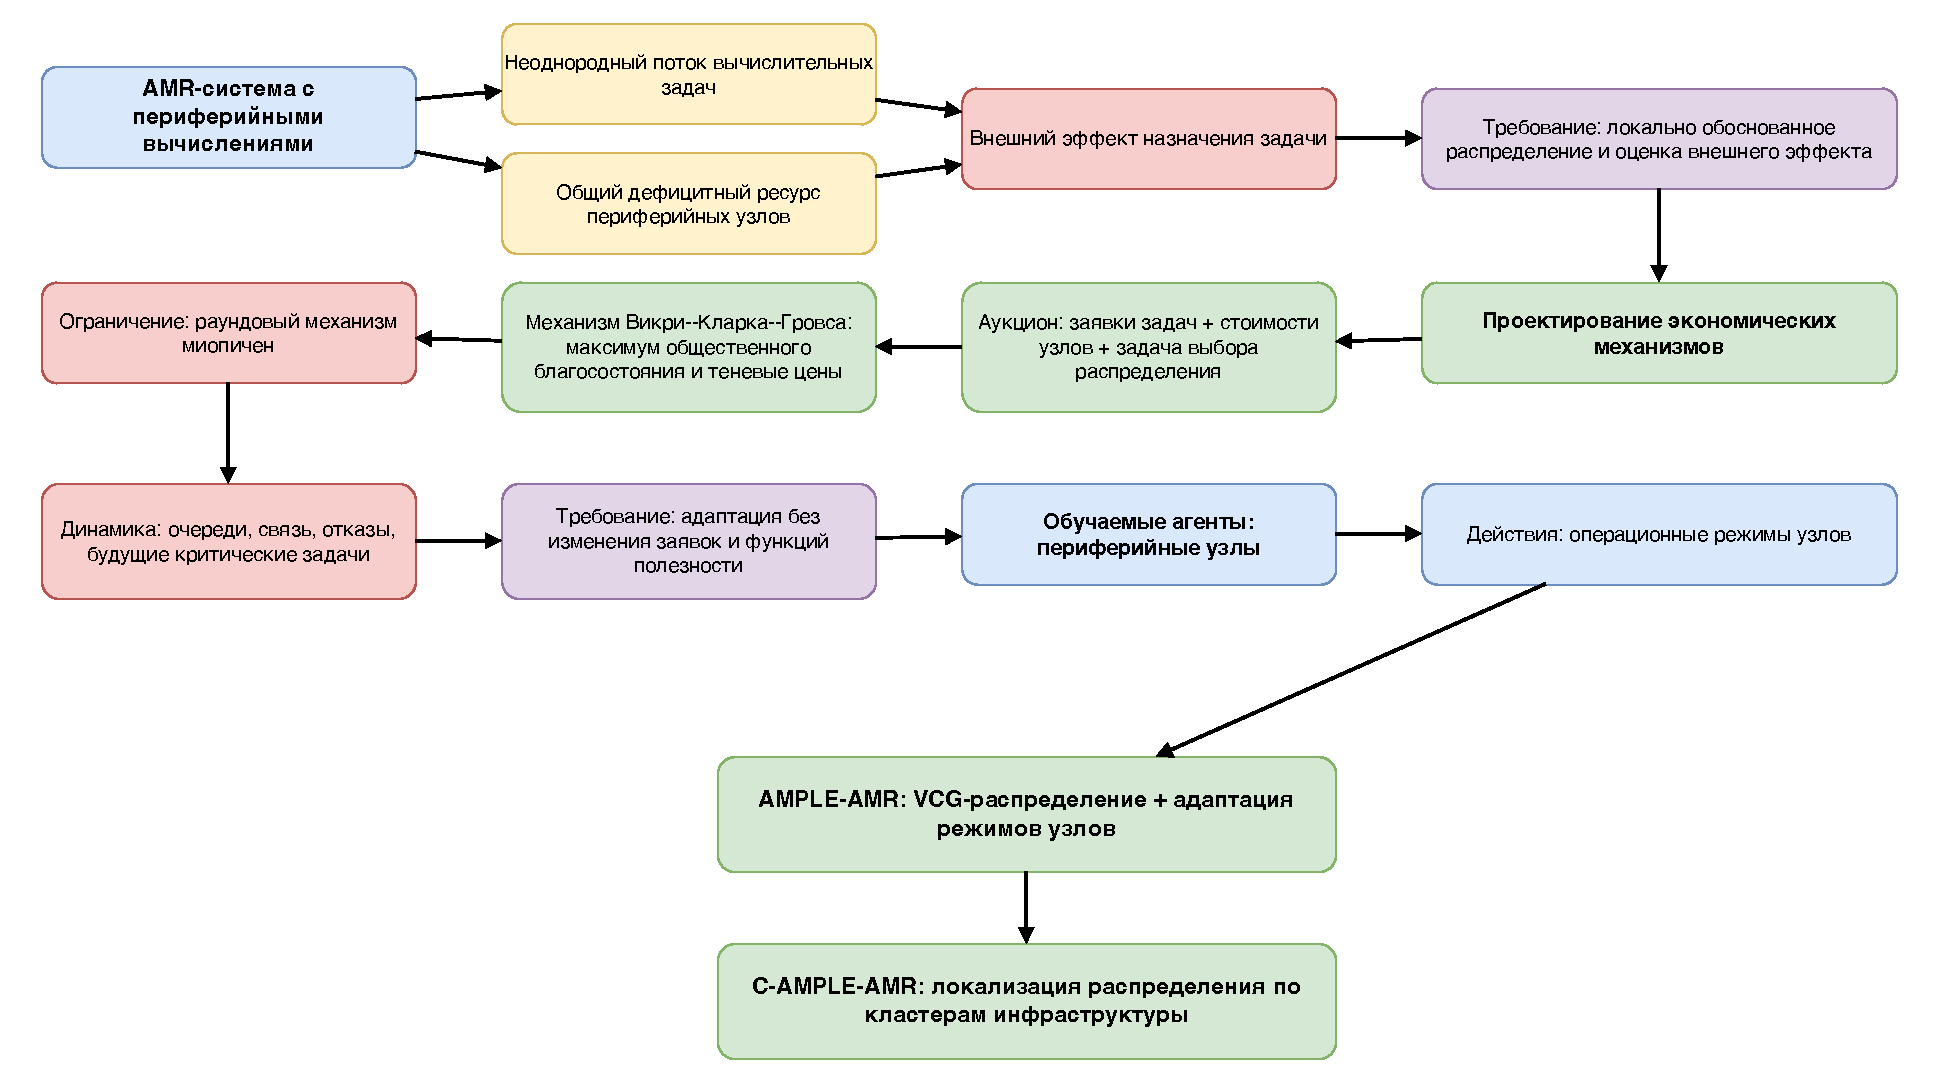
\includegraphics[width=0.95\textwidth]{ch1_method_logic}
	\caption{Логика выбора гибридного метода распределения вычислительных задач}
	\label{img:ch1_method_logic}
\end{figure}

\section{Метод AMPLE-AMR}

Архитектура метода \methodname{} (\textit{Adaptive Multi-agent Policy Learning with Edge Auctions for Autonomous Mobile Robots}) построена как двухуровневый контур принятия решений. Верхний, обучаемый, уровень не распределяет задачи напрямую. Он выбирает операционные режимы периферийных узлов: например, консервативный режим, нормальный режим, агрессивное раскрытие емкости, резервирование ресурсов или критический режим обслуживания. Режим изменяет экспонируемую емкость узла, правила допуска задач, приоритеты обслуживания и степень защиты от перегрузки. Нижний уровень получает уже сформированные ограничения и решает задачу распределения задач в текущем раунде.

\begin{figure}[H]
	\centering
	\safeincludegraphics[width=0.96\textwidth]{ch5_ample_amr_concept.pdf}
	\caption{Концептуальная схема метода \methodname{}: обучаемое управление режимами задает условия распределения, а аукционный слой выполняет назначение задач.}
	\label{fig:ample-concept}
\end{figure}

Такое разделение позволяет сохранить интерпретируемость распределения. \textbf{Роботы} формируют заявки и оценки ценности задач; \textbf{периферийные узлы} задают ограничения и стоимость обслуживания; \textbf{аукционный слой} выбирает распределение; \textbf{обучаемая политика} лишь изменяет режимы работы инфраструктуры. Она не подменяет заявки роботов и не учится стратегически искажать оценки ценности. Это существенно снижает риск того, что многоагентное обучение разрушит смысл аукционного механизма.

\begin{figure}[H]
	\centering
	\safeincludegraphics[width=0.95\textwidth]{ch5_ample_architecture.pdf}
	\caption{Архитектура метода: поток задач проходит через контур режимов, ограничения узлов и слой распределения.}
	\label{fig:ample-architecture}
\end{figure}

Аукционный слой является VCG-подобным. В каждом раунде он решает задачу выбора распределения, максимизируя общественное благосостояние (Social Welfare)~\cite{Arrow2011SocialWelfareHandbook}. Для назначенной задачи вычисляется внутренний платеж, отражающий \textbf{внешний эффект}: насколько присутствие данной задачи ухудшает или изменяет доступность ресурса для остальных задач. В работе эти платежи не трактуются как реальные денежные переводы. Их роль --- внутренняя диагностика дефицита ресурса и формальная фиксация того, что задача использует общий ограниченный ресурс не изолированно, а в конкуренции с другими задачами.

Свойства VCG-подобного слоя зафиксированы локально. Эффективность, индивидуальная рациональность и стратегическая совместимость могут обсуждаться только для одного статического раунда при фиксированных режимах узлов, корректных оценках полезности, корректной модели стоимости и точном решении задачи выбора победителей. Эти свойства не переносятся автоматически на повторяющуюся систему с обучением, очередями, изменением нагрузки и частичной наблюдаемостью. Такое ограничение принципиально: метод использует подход <<проектирование экономических механизмов>> как строгий локальный слой, но не выдает динамическую систему за классический однораундовый VCG-аукцион.

Долгосрочная адаптация вынесена в кооперативное многоагентное обучение с подкреплением (MARL). Задача управления режимами формализована как децентрализованный частично наблюдаемый марковский процесс принятия решений (Dec-POMDP). \textbf{Агентами} являются периферийные узлы; \textbf{локальные наблюдения} включают загрузку, длину очереди, статистику задержек, признаки сетевой связности, историю принятых задач и предыдущий режим. \textbf{Командное вознаграждение} связывается с общественным благосостоянием, качеством обслуживания, нарушениями дедлайнов и перегрузкой. Для обучения выбран \textbf{QMIX}, поскольку он соответствует парадигме централизованного обучения и децентрализованного исполнения: на этапе обучения используется глобальная информация, а в эксплуатации каждый узел выбирает действие по локальному наблюдению~\cite{Oliehoek2016DecPOMDP,Amato2024CTDE,Sunehag2017VDN,Rashid2018QMIX}.

Для крупных конфигураций предложен вариант \clustermethodname{}. Он разбивает граф периферийной инфраструктуры на кластеры и проводит распределение локально внутри кластеров~\cite{Karypis1998Metis,Blondel2008Louvain}. Идея состоит в том, чтобы уменьшить вычислительные и коммуникационные накладные расходы глобального распределения. Однако кластеризация неизбежно вводит компромисс: локальные аукционы дешевле, но могут терять часть общественного благосостояния из-за ограничения пространства допустимых назначений.

\section{Математическая формализация метода}

\subsection{Модель распределения вычислительных задач}

Рассматривается локальная система одного оператора, в которой множество автономных мобильных роботов и множество периферийных узлов задаются как
\begin{equation}
	\mathcal{R}=\{r_1,r_2,\ldots,r_m\},\qquad
	\mathcal{N}=\{n_1,n_2,\ldots,n_k\}
	\label{eq:nir_sets}
\end{equation}
и функционируют в дискретном времени.

\textbf{Робот} $r_i$ в раунде $t$ формирует множество задач $\mathcal{T}_i(t)$, а совокупный входной поток текущего раунда равен
\begin{equation}
	\mathcal{T}(t)=\bigcup_{i=1}^{m}\mathcal{T}_i(t).
	\label{eq:nir_all_tasks}
\end{equation}
\textbf{Задача} $\tau\in\mathcal{T}_i(t)$ описывается вектором
\begin{equation}
	\tau=\bigl(i,c_{\tau},b^{in}_{\tau},b^{out}_{\tau},q^{cpu}_{\tau},q^{mem}_{\tau},q^{gpu}_{\tau},\Delta_{\tau},\pi_{\tau},t^{arr}_{\tau}\bigr),
	\label{eq:nir_task_vector}
\end{equation}
где $i$ --- индекс робота-источника, $c_\tau$ --- класс задачи, $b^{in}_\tau$ и $b^{out}_\tau$ --- объемы входных и выходных данных, $q^r_\tau$ --- требование к ресурсу $r\in\{cpu,mem,gpu\}$, $\Delta_\tau$ --- допустимый срок обработки, $\pi_\tau$ --- приоритет, $t^{arr}_\tau$ --- момент поступления задачи.

\textbf{Периферийный узел} $n_j\in\mathcal{N}$ характеризуется полной ресурсной емкостью
\begin{equation}
	\mathrm{Cap}_j=\bigl(C^{cpu}_j,C^{mem}_j,C^{gpu}_j\bigr),
	\label{eq:nir_capacity}
\end{equation}
текущей нагрузкой
\begin{equation}
	L_j(t)=\bigl(L^{cpu}_j(t),L^{mem}_j(t),L^{gpu}_j(t)\bigr),
	\label{eq:nir_load}
\end{equation}
физически свободной емкостью
\begin{equation}
	A_j(t)=\mathrm{Cap}_j-L_j(t),
	\label{eq:nir_available}
\end{equation}
очередью $Q_j(t)$ и индикатором отказа $f_j(t)\in\{0,1\}$. \textbf{Операционный режим} узла обозначается как
\begin{equation}
	\kappa_j(t)\in\mathcal{K}_j,
	\label{eq:nir_mode}
\end{equation}
а совместный вектор режимов --- как $\kappa(t)=(\kappa_1(t),\ldots,\kappa_k(t))$ или, короче, $\kappa_t$. Режим не меняет заявки роботов и функции полезности, а задает экспонируемую емкость узла:
\begin{equation}
	\bar{A}^{r}_j(t,\kappa_j)=\eta^{r}_j(\kappa_j)\bigl(C^{r}_j-L^{r}_j(t)\bigr),
	\quad r\in\{cpu,mem,gpu\},
	\label{eq:nir_exposed_capacity}
\end{equation}
где $\eta^r_j(\kappa_j)\in[0,1]$ --- коэффициент экспонирования ресурса в выбранном режиме.

Для пары робот--узел используется индикатор достижимости $a_{ij}(t)$. Если задача $\tau$ робота $r_{i(\tau)}$ назначается на узел $n_j$, ее \textbf{полное ожидаемое время выполнения} задается как
\begin{equation}
	T_{\tau j}(t)=T^{net}_{i(\tau)j,\tau}(t)+T^{queue}_{j}(t)+T^{proc}_{\tau j}(t),
	\label{eq:nir_task_time}
\end{equation}
где сетевая составляющая определяется выражением
\begin{equation}
	T^{net}_{ij,\tau}(t)=d_{ij}(t)+\frac{b^{in}_{\tau}}{B^{up}_{ij}(t)+\varepsilon}+\frac{b^{out}_{\tau}}{B^{down}_{ji}(t)+\varepsilon}.
	\label{eq:nir_network_time}
\end{equation}
Здесь $d_{ij}(t)$ --- базовая задержка канала, $B^{up}_{ij}(t)$ и $B^{down}_{ji}(t)$ --- пропускные способности восходящего и нисходящего каналов, $\varepsilon>0$ --- малая константа.

\textbf{Полезность назначения} задачи на узел задается как
\begin{equation}
	U_i(\tau,n_j,t)=V_i(\tau)\psi_{c_{\tau}}(T_{\tau j}(t),\Delta_{\tau})-E^{tx}_{i\tau j}(t)-P^{viol}_{\tau j}(t),
	\label{eq:nir_utility}
\end{equation}
где $V_i(\tau)$ --- базовая ценность задачи для робота-источника, $\psi_{c_\tau}$ --- функция деградации полезности при задержке, $E^{tx}_{i\tau j}(t)$ --- энергетические затраты передачи, $P^{viol}_{\tau j}(t)$ --- штраф за нарушение срока. 

\textbf{Стоимость выполнения задачи} на узле записывается как
\begin{equation}
	C_j(\tau,r_{i(\tau)},t)=C^{comp}_j(\tau)+C^{net}_j(\tau,r_{i(\tau)},t)+C^{over}_j(\tau,t)+C^{rel}_j(t).
	\label{eq:nir_cost}
\end{equation}
\textbf{Чистый вклад назначения} определяется выражением
\begin{equation}
	g_{\tau j}(t)=U_{i(\tau)}(\tau,n_j,t)-C_j(\tau,r_{i(\tau)},t).
	\label{eq:nir_assignment_gain}
\end{equation}

\textbf{Распределение задач} описывается бинарными переменными
\begin{equation}
	x_{\tau j}(t)=
	\begin{cases}
		1, & \text{если задача } \tau \text{ назначена узлу } n_j,\\
		0, & \text{иначе.}
	\end{cases}
	\label{eq:nir_assignment_var}
\end{equation}
\textbf{Множество допустимых распределений} $\mathcal{X}(t,\kappa(t))$ задается ограничениями единственности назначения, ресурсной емкости, достижимости, отказа и, для задач с жестким сроком, времени выполнения:
\begin{align}
	&\sum_{j=1}^{k}x_{\tau j}(t)\leq 1, &&\forall \tau\in\mathcal{T}(t),
	\label{eq:nir_single_assignment}\\
	&\sum_{\tau\in\mathcal{T}(t)}x_{\tau j}(t)q^r_{\tau}\leq \bar{A}^{r}_{j}(t,\kappa_j), &&\forall n_j\in\mathcal{N},\; r\in\{cpu,mem,gpu\},
	\label{eq:nir_capacity_constraint}\\
	&x_{\tau j}(t)\leq a_{i(\tau)j}(t), &&\forall \tau\in\mathcal{T}(t),\; \forall n_j\in\mathcal{N},
	\label{eq:nir_reachability_constraint}\\
	&x_{\tau j}(t)\leq 1-f_j(t), &&\forall \tau\in\mathcal{T}(t),\; \forall n_j\in\mathcal{N},
	\label{eq:nir_failure_constraint}\\
	&x_{\tau j}(t)T_{\tau j}(t)\leq \Delta_{\tau}, &&\forall \tau: c_{\tau}\in\mathcal{C}^{hard}.
	\label{eq:nir_deadline_constraint}
\end{align}

\subsection{Аукционный слой}

\textbf{Общественное благосостояние} текущего раунда определяется как сумма чистых вкладов назначений:
\begin{equation}
	SW(x,t)=\sum_{\tau\in\mathcal{T}(t)}\sum_{j=1}^{k}x_{\tau j}(t)g_{\tau j}(t).
	\label{eq:nir_social_welfare}
\end{equation}
При фиксированных режимах периферийных узлов аукционный слой решает \textbf{задачу выбора распределения}:
\begin{equation}
	x^*(t)\in\arg\max_{x\in\mathcal{X}(t,\kappa(t))}SW(x,t).
	\label{eq:nir_wdp}
\end{equation}
Эта задача является однораундовой задачей выбора победителей: она максимизирует качество текущего распределения, но не отвечает за долговременное изменение очередей, отказов и будущей нагрузки.

Для записи VCG-подобных платежей вводится множество участников $\mathcal{H}=\mathcal{R}\cup\mathcal{N}$. Вклад робота $r_i$ в общественное благосостояние обозначается как $v_{r_i}(x,t)=V_i(x,t)$, а вклад узла $n_j$ --- как $v_{n_j}(x,t)=-C_j(x,t)$. Тогда
\begin{equation}
	SW(x,t)=\sum_{h\in\mathcal{H}}v_h(x,t).
	\label{eq:nir_sw_by_agents}
\end{equation}
Для участника $h\in\mathcal{H}$ максимальное благосостояние остальных участников при исключении $h$ равно
\begin{equation}
	SW^*_{-h}(t)=\max_{x\in\mathcal{X}_{-h}(t,\kappa(t))}\sum_{\ell\in\mathcal{H},\ell\neq h}v_{\ell}(x,t).
	\label{eq:nir_without_h}
\end{equation}
\textbf{VCG-подобный платеж}, взимаемый с участника $h$, определяется как
\begin{equation}
	p_h(t)=SW^*_{-h}(t)-\sum_{\ell\in\mathcal{H},\ell\neq h}v_{\ell}(x^*(t),t).
	\label{eq:nir_vcg_payment}
\end{equation}
Положительное значение $p_h(t)$ означает внутреннее списание, отрицательное --- внутреннюю компенсацию. В рамках данной работы платеж не является коммерческим переводом; он используется как внутренняя теневая цена внешнего эффекта.

\subsection{Адаптивное многоагентное управление}

Управление режимами периферийных узлов формализуется как децентрализованный частично наблюдаемый марковский процесс принятия решений (\textbf{Dec-POMDP})
\begin{equation}
	\mathcal{M}^{ctrl}=\left\langle \mathcal{A},\mathcal{S},\{\mathcal{O}_j\}_{j=1}^{k},\{\mathcal{K}_j\}_{j=1}^{k},P,R,\Omega,\gamma\right\rangle,
	\label{eq:nir_decpomdp}
\end{equation}
где $\mathcal{A}=\{a_1,\ldots,a_k\}$ --- множество обучаемых агентов, соответствующих периферийным узлам, $\mathcal{S}$ --- множество глобальных состояний, $\mathcal{O}_j$ --- пространство локальных наблюдений агента, $\mathcal{K}_j$ --- множество режимов узла, $P(s_{t+1}\mid s_t,\kappa_t)$ --- функция переходов, $R(s_t,\kappa_t,s_{t+1})$ --- командная функция вознаграждения, $\Omega$ --- функция наблюдений, $\gamma$ --- коэффициент дисконтирования. Совместное действие имеет вид
\begin{equation}
	\kappa_t=\bigl(\kappa_1(t),\ldots,\kappa_k(t)\bigr),\qquad \kappa_j(t)\in\mathcal{K}_j.
	\label{eq:nir_joint_action}
\end{equation}

В базовой дискретной постановке множество режимов задаётся как
\begin{equation}
	\mathcal{K}_j =
	\{
	\kappa^{safe},
	\kappa^{normal},
	\kappa^{aggressive},
	\kappa^{reserve},
	\kappa^{critical}
	\}.
	\label{eq:ch4_action_set}
\end{equation}

Режим $\kappa^{safe}$ соответствует защитному поведению: узел ограничивает приём новых задач при высокой загрузке, риске нарушения сроков или признаках деградации. Режим $\kappa^{normal}$ соответствует штатной работе с умеренным экспонированием свободной ёмкости. Режим $\kappa^{aggressive}$ соответствует расширенному приёму задач при благоприятном состоянии узла и низкой очереди. Режим $\kappa^{reserve}$ сохраняет часть ёмкости для возможных будущих критических задач. Режим $\kappa^{critical}$ отдаёт предпочтение задачам, связанным с безопасностью, локализацией, обходом препятствий и срочным перепланированием.

\textbf{Глобальное состояние} может быть записано как
\begin{equation}
	s_t=\left(G(t),\{L_j(t)\}_{j=1}^{k},\{Q_j(t)\}_{j=1}^{k},\{F_j(t)\}_{j=1}^{k},\mathcal{T}(t),\{d_{ij}(t)\}_{i,j},Z_t\right),
	\label{eq:nir_state}
\end{equation}
а локальное наблюдение агента $a_j$ --- как
\begin{equation}
	o^j_t=\Omega_j(s_t)=\left(o^{j,tech}_t,g^j_t\right),
	\label{eq:nir_observation}
\end{equation}
где $o^{j,tech}_t$ содержит технические признаки узла, а $g^j_t$ --- агрегированные аукционные признаки предыдущего распределения: платежи, оценки внешнего эффекта, использование экспонируемой емкости и вклад назначенных задач в $SW$. Локальная история задается как $h^j_t$, а политика агента имеет вид
\begin{equation}
	\pi_j(\kappa_j\mid h^j_t).
	\label{eq:nir_local_policy}
\end{equation}

\textbf{Командное вознаграждение} согласует обучение с качеством распределения и эксплуатационной устойчивостью системы:
\begin{equation}
	r_t=\alpha_{sw}\widetilde{SW}(t)-\alpha_{viol}\mathrm{Viol}(t)-\alpha_{drop}\mathrm{Drop}(t)-\alpha_{wait}\mathrm{Wait}(t)-\alpha_{imb}\mathrm{Imb}(t)-\alpha_{over}\mathrm{Over}(t).
	\label{eq:nir_reward}
\end{equation}
Здесь $\widetilde{SW}(t)$ --- нормированное общественное благосостояние, $\mathrm{Viol}(t)$ --- доля задач с нарушенными сроками, $\mathrm{Drop}(t)$ --- доля отклоненных или нераспределенных задач, $\mathrm{Wait}(t)$ --- нормированное среднее ожидание, $\mathrm{Imb}(t)$ --- дисбаланс загрузки, $\mathrm{Over}(t)$ --- штраф за перегрузку.

\textbf{В алгоритме QMIX} локальные функции ценности периферийных узлов объединяются в совместную функцию
\begin{equation}
	Q_{tot}(s_t,\kappa_t)=f_{mix}\left(Q_1(h^1_t,\kappa_1),\ldots,Q_k(h^k_t,\kappa_k),s_t\right),
	\label{eq:nir_qmix_total}
\end{equation}
при условии монотонности
\begin{equation}
	\frac{\partial Q_{tot}}{\partial Q_j}\geq 0,\qquad j=1,\ldots,k.
	\label{eq:nir_qmix_monotonicity}
\end{equation}
Функция потерь имеет вид
\begin{equation}
	\mathcal{L}(\theta)=\mathbb{E}_{e_t\sim\mathcal{B}}\left[\left(y_t-Q_{tot}(s_t,\kappa_t;\theta)\right)^2\right],
	\label{eq:nir_qmix_loss}
\end{equation}
где
\begin{equation}
	y_t=\tilde{r}_t+\gamma(1-done_t)\max_{\kappa'_{t+1}}Q^{-}_{tot}(s_{t+1},\kappa'_{t+1}).
	\label{eq:nir_qmix_target}
\end{equation}

Итоговый шаг метода AMPLE-AMR записывается как композиция обучаемого и аукционного слоев:
\begin{equation}
	\kappa_t=\pi_{\theta}(\{h^j_t\}_{j=1}^{k}),\qquad
	x^*(t)=\operatorname{Auction}(\mathcal{T}(t),\mathcal{N},\kappa_t),\qquad
	p(t)=\operatorname{VCG}(x^*(t)).
	\label{eq:nir_hybrid_step}
\end{equation}
Тем самым обучаемая политика управляет не назначениями задач и не ставками роботов, а режимами периферийных узлов. Аукционный слой сохраняет роль интерпретируемого однораундового распределителя, а многоагентное обучение отвечает за адаптацию ресурсного контекста во времени.

\section{Программная реализация}

Программный прототип метода AMPLE-AMR~\cite{Tereschenko2026AMPLEAMRPrototype} включает генератор складских сценариев, модели роботов и периферийных узлов, сетевую модель, генератор вычислительных задач, эвристическое распределение, VCG-подобное распределение, кластерное распределение, контур обучения QMIX, сценарии экспериментального запуска и экспорт результатов в CSV, графики и LaTeX-таблицы.

\begin{figure}[h]
	\centering
	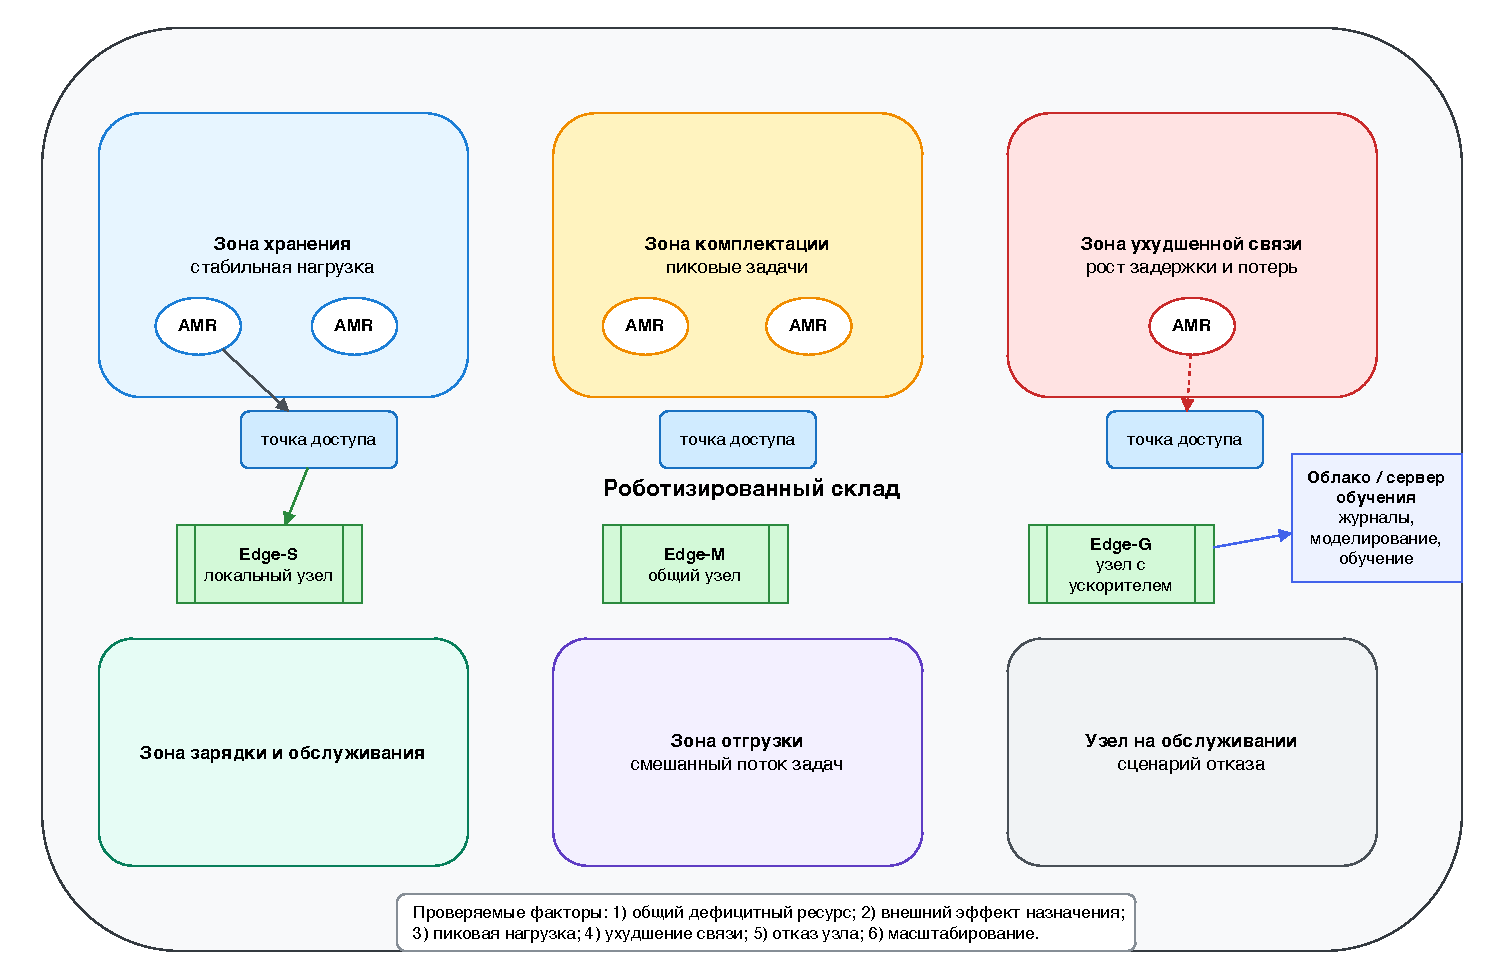
\includegraphics[width=0.95\textwidth]{ch6_warehouse_scenario}
	\caption{Складская среда с автономными мобильными роботами, периферийными узлами и зонами изменения нагрузки}
	\label{img:ch6_warehouse_scenario}
\end{figure}

В качестве прикладного домена выбран \textbf{роботизированный склад}~\cite{Fragapane2021AMRPlanning,Fragapane2024AMRMaterialHandling,Lackner2024AMRIntralogistics,Keith2024WarehouseAMRReview}. Этот домен удобен не только как иллюстрация, но и как содержательно подходящая область применения: роботы работают в локальной зоне, инфраструктура может быть размещена вблизи склада, поток задач неоднороден, а качество обслуживания зависит от задержек и устойчивости к перегрузкам. В экспериментах используются сценарии стабильной нагрузки, пиковой нагрузки, разнородной периферийной инфраструктуры, деградации связи, отказов узлов, масштабирования и чувствительности к параметрам операционных режимов.

Сравнение проводится между пятью вариантами: \textbf{Fixed-Heuristic}, \textbf{Fixed-VCG}, \textbf{QMIX-Heuristic}, \textbf{AMPLE-AMR} и \textbf{C-AMPLE-AMR}. Такая матрица позволяет разложить вклад метода на компоненты. Fixed-Heuristic является простым базисом. Fixed-VCG проверяет, дает ли выигрыш сам VCG-подобный слой при фиксированных режимах. QMIX-Heuristic проверяет вклад обучаемого выбора режимов без VCG-подобного распределения. AMPLE-AMR проверяет их совместное использование. C-AMPLE-AMR проверяет цену и пользу кластеризации.

Основные метрики включают общественное благосостояние, долю обслуженных задач, долю отклоненных задач, долю нарушений дедлайнов, 95-й квантиль задержки, загрузку узлов, дисбаланс загрузки и накладные расходы принятия решения. Отдельно анализируются внутренние платежи и оценки внешнего эффекта как диагностические признаки дефицита ресурса.

\section{Результаты экспериментальной проверки}

Экспериментальная проверка показала, что обучаемая политика режимов не вырождается в постоянный выбор одного режима. В пиковом сценарии политика почти полностью переходит к режимам \texttt{critical} и \texttt{reserve}, что соответствует ожидаемой реакции на рост входного потока задач. Это важный результат: выигрыш метода связан не с формальным наличием нескольких режимов, а с тем, что политика действительно меняет режимы в зависимости от состояния среды.

\begin{figure}[H]
\centering
\safeincludegraphics[width=0.92\textwidth]{ch8_operation_mode_distribution.pdf}
\caption{Распределение операционных режимов периферийных узлов по экспериментальным сценариям.}
\label{fig:operation-modes}
\end{figure}

Сводные результаты показывают устойчивое преимущество AMPLE-AMR относительно фиксированного базиса по общественному благосостоянию во всех основных сценариях. При стабильной нагрузке выигрыш составляет $+124.0$ условных единицы, при пиковой нагрузке $+210.5$, в разнородной инфраструктуре $+95.6$, при деградации связи $+94.9$, при отказах узлов $+110.7$. Одновременно снижается хвостовая задержка: например, в пиковом сценарии 95-й квантиль уменьшается с $75.2$ до $50.9$ мс, а при отказах узлов --- с $60.2$ до $50.2$ мс.

\begin{table}[H]
\centering
\caption{Ключевые результаты AMPLE-AMR относительно Fixed-Heuristic}
\label{tab:key-results}
\begin{tabular}{lrrrr}
\toprule
Сценарий & $SW$ Fixed-H & $SW$ AMPLE & $\Delta SW$ & $\Delta P95$, мс \\
\midrule
Стабильная нагрузка & 1062.5 & 1186.5 & +124.0 & -17.5 \\
Пиковая нагрузка & 1608.6 & 1819.1 & +210.5 & -24.2 \\
Разнородные узлы & 1207.9 & 1303.5 & +95.6 & -8.6 \\
Деградация связи & 824.2 & 919.1 & +94.9 & -4.3 \\
Отказы узлов & 980.2 & 1090.9 & +110.7 & -10.0 \\
\bottomrule
\end{tabular}
\end{table}

\begin{figure}[H]
\centering
\safeincludegraphics[width=0.92\textwidth]{ch8_welfare_by_scenario.pdf}
\caption{Общественное благосостояние по сценариям экспериментальной проверки.}
\label{fig:welfare-by-scenario}
\end{figure}

Главный содержательный вывод состоит в том, что в текущей реализации доминирующий вклад дает обучаемый выбор операционных режимов. AMPLE-AMR и QMIX-Heuristic во многих глобальных сценариях показывают близкие или совпадающие интегральные метрики, тогда как Fixed-VCG практически не отделяется от Fixed-Heuristic. Это не обесценивает аукционный слой, но уточняет его роль: в текущей параметризации он не является основным источником численного выигрыша, а прежде всего задает интерпретируемую структуру распределения и диагностические сигналы внешнего эффекта.

Проверка внутренних цен показывает умеренный результат. Оценки внешнего эффекта возрастают в стрессовых состояниях, но их корреляция с загрузкой узлов остается слабой. Следовательно, внутренние платежи можно использовать как дополнительный диагностический признак дефицита ресурса, но не как единственный управляющий сигнал. Для практического управления они должны комбинироваться с более устойчивыми признаками: загрузкой узлов, длиной очереди, задержкой, долей отклоненных задач и нарушениями дедлайнов.

Масштабируемая версия C-AMPLE-AMR также дала неоднозначный результат. На малых и средних конфигурациях кластеризация не окупается: накладные расходы могут увеличиваться, а качество распределения ухудшается. На экстремальном масштабе Warehouse-XL кластерный вариант уменьшает суммарные накладные расходы примерно с $98.7$ до $50.5$ мс, то есть почти вдвое, но ценой потери общественного благосостояния на $32.8$ условных единицы. Поэтому C-AMPLE-AMR следует рассматривать как перспективный задел для масштабирования, а не как полностью завершенное универсальное решение.

\begin{figure}[H]
\centering
\safeincludegraphics[width=0.92\textwidth]{ch8_overhead_scalability.pdf}
\caption{Накладные расходы распределения при масштабировании.}
\label{fig:overhead-scalability}
\end{figure}

\section{Научный вклад и ограничения}

Основной научный результат исследования состоит в разработке гибридной архитектуры распределения вычислительных задач, где механизм-дизайн и многоагентное обучение используются не как взаимозаменяемые инструменты, а как слои с разными функциями. VCG-подобный слой отвечает за локально интерпретируемое распределение ограниченного ресурса и расчет внутреннего внешнего эффекта. Кооперативное обучение отвечает за изменение режима инфраструктуры в зависимости от динамики среды. Такое разделение позволяет избежать прямого обучения заявок и сохранить смысл аукционного распределения.

К числу полученных результатов относятся: математическая модель AMR-системы с периферийной инфраструктурой; формализация распределения задач как задачи внутренней координации общего дефицитного ресурса; VCG-подобный слой с интерпретацией платежей как теневых цен; Dec-POMDP-постановка задачи управления режимами узлов; метод AMPLE-AMR; кластерный вариант C-AMPLE-AMR; программный прототип и воспроизводимый экспериментальный контур.

Вместе с тем исследование не скрывает ограничений. Во-первых, сильная гипотеза о самостоятельном преимуществе VCG-подобного распределения над жадкой эвристикой при фиксированных режимах в текущих экспериментах не подтверждена. Во-вторых, AMPLE-AMR пока не демонстрирует устойчивого дополнительного выигрыша относительно QMIX-Heuristic, если сравнивать только интегральные метрики. В-третьих, внутренние цены пока являются вспомогательным, а не основным диагностическим сигналом. В-четвертых, кластерная версия требует дальнейшей оптимизации локальных аукционов и стратегии разбиения графа.

Эти ограничения важны для корректной интерпретации диссертационного результата. Работа показывает не то, что VCG-слой автоматически улучшает любое распределение, а то, что гибридная архитектура позволяет формально разделить распределение ресурса и адаптацию инфраструктуры. Практический эффект в текущей реализации достигается главным образом за счет обучаемого управления режимами, тогда как аукционный слой обеспечивает структурную и диагностическую основу для дальнейшего развития метода.

\section{Заключение}

В ходе научно-исследовательской работы разработан и экспериментально проверен метод адаптивного распределения вычислительных задач автономных мобильных роботов в системах периферийных вычислений. Полученная диссертационная конструкция включает предметную модель, математическую постановку, VCG-подобный аукционный слой, Dec-POMDP-формализацию управления режимами, QMIX-контур обучения, метод AMPLE-AMR, кластерную модификацию C-AMPLE-AMR, программный прототип и набор воспроизводимых экспериментов.

Эксперименты в домене роботизированного склада подтверждают, что адаптивное управление операционными режимами периферийных узлов повышает устойчивость системы при стабильной нагрузке, пиковом потоке задач, деградации связи и отказах. Наиболее сильный эффект проявляется в росте общественного благосостояния и снижении 95-го квантиля задержки. При этом результаты уточняют исходную гипотезу: основной численный выигрыш дает обучаемый контур, а VCG-подобный слой в текущей реализации играет преимущественно структурную и диагностическую роль. Такая интерпретация делает итог исследования более точным и задает понятный план дальнейшей работы: усилить различие между эвристическим и VCG-подобным распределением, доработать использование внутренних цен в обучаемом контуре и оптимизировать кластерную версию для крупных инфраструктур.

\begingroup
\sloppy
\bibliographystyle{BibTeX-Styles/ugost2008}
\bibliography{biblio/external,biblio/author,biblio/registered}
\endgroup

\end{document}
